% -*- latex -*-
%%%%%%%%%%%%%%%%%%%%%%%%%%%%%%%%%%%%%%%%%%%%%%%%%%%%%%%%%%%%%%%%
%%%%
%%%% This TeX file is part of the course
%%%% Introduction to Scientific Programming in C++/Fortran2003
%%%% copyright 2017/8 Victor Eijkhout eijkhout@tacc.utexas.edu
%%%%
%%%% loop.tex : loop constructs
%%%%
%%%%%%%%%%%%%%%%%%%%%%%%%%%%%%%%%%%%%%%%%%%%%%%%%%%%%%%%%%%%%%%%

\Level 0 {Basic `for' statement}
\label{sec:for}

There are many cases where you want to repeat an operation or series
of operations:
\begin{itemize}
\item A time-dependent numerical simulation executes a fixed number of
  steps, or until some stoping test.
\item Recurrences: \[ x_{i+1} = f(x_i). \]
\item Inspect or transformation every element of a database table.
\end{itemize}

\begin{remark}
  The first two cases actually need to be performed in
  sequence, while the last one corresponds more to a mathematical
  `forall' quantor. This difference can be exploited when you learn
  \indextermsub{parallel}{programming}. Fortran has a
  \indextermbus{do}{concurrent} loop construct for this.
\end{remark}

What you need is known as a~\indextermdef{loop}: a~number of
statements that get repeated. The two types of loop statement in C++ are:
\begin{itemize}
\item the \indextermsub{for}{loop} which is typically associated with
  a pre-determined number of repetitions, and with the repeated
  statements being based on a counter of some sort; and
\item the \indextermsub{while}{loop}, where the statements are
  repeated indefinitely until some condition is satisfied.
\end{itemize}
We will now consider the for loop; the while loop comes in
section~\ref{sec:loopuntil}.

In the most common case, a for loop has a
\indextermbus{loop}{counter}, ranging from some lower to some upper
bound. An example showing the syntax for this simple case is:
\begin{verbatim}
for (int var=low; var<upper; var++) {
  // statements involving the loop variable:
  cout << "The square of " << var << " is " << var*var << endl;
}
\end{verbatim}
The \n{for} line is called the \indextermbus{loop}{header}, and the
statements between curly brackets the \indextermbus{loop}{body}.

\begin{slide}{Repeat statement}
  \label{sl:for}
  Sometimes you need to repeat a statement a number of times. That's
  where the \indextermdef{loop} comes in. A~loop has a counter, called
  a~\indexterm{loop variable}, which (usually) ranges from a lower bound
  to an upper bound.

  Here is the syntax in the simplest case:
\begin{verbatim}
for (int var=low; var<upper; var++) {
  // statements involving var
  cout << "The square of " << var << " is " << var*var << endl;
}
\end{verbatim}
\begin{cnote}
Use compiler flag \n{-std=c99}.
\end{cnote}
\end{slide}

\begin{exercise}
  \label{ex:manyhello}
  Read an integer value with \n{cin}, and print `Hello world' that many times.
\end{exercise}

The loop header has three components, all of which are optional.
\begin{itemize}
\item An initialization. This is usually a declaration and
  initialization of an integer \indextermbus{loop}{variable}. Using
  floating point values is less advisable.
\item A stopping test, usually
  involving the loop variable. If you leave this out, you need a
  different mechanism for stopping the loop; see~\ref{sec:loopuntil}.
\item An increment, often~\n{i++} or spelled out \n{i=i+1}. You can let the loop count down by using~\n{i--}.
\end{itemize}

Some variations on the simple case.
\begin{itemize}
\item The loop variable can be defined outside the loop:
\begin{verbatim}
int var;
for (var=low; var<upper; var++) {
\end{verbatim}
but it's cleaner to make it local. However:
\begin{verbatim}
int var;
... code that sets var ...
for ( ; var<upper; var++) {
  ... loop body ...
}
... code that uses the final value of var ...
\end{verbatim}
\item The stopping test can be omitted
\begin{verbatim}
for (int var=low; ; var++) { ... }
\end{verbatim}
if the loops ends in some other way. You'll see this later.
\item The stopping test doesn't need to be an upper bound. Here is an
  example of a loop that counts down to a lower bound.
\begin{verbatim}
for (int var=high; var>=low; var--) { ... }
\end{verbatim}
\item Here are a couple of popular increments:
  \begin{itemize}
  \item \n{i++} for a loop that counts forward;
  \item \n{i--} for a loop that counts backward;
  \item \n{i+=2} to cover only odd or even numbers, depending on
    where you started;
  \item \n{i*=10} to cover powers of ten.
  \end{itemize}
\item The test is performed before each iteration:
  \snippetwithoutput{pretest}{basic}{pretest}
  (Historical note: at some point Fortran was post-test)
\item The loop body can be a single statement:
\begin{verbatim}
if (x<0)
  x = -x;
\end{verbatim}
or a block:
\begin{verbatim}
if (x<0) {
  cout << "Error" << endl;
  x = -x;
}
\end{verbatim}
\end{itemize}

\begin{slide}{Loop syntax}
  \label{sl:for-syntax}
  \begin{itemize}
  \item Loop variable is usually an integer.
  \item The stopping test be any test; can even be empty.
  \item The stopping test is performed at the start of each iteration.
  \item The increment can be a decrement or something like \n{var*=10}
  \item Any and all of initialization, test, increment can be empty:\\
    \n{for(;;) {...}}
  \item (The loop variable can be defined outside the loop:
\begin{verbatim}
int var;
for (var=low; var<upper; var++) {
\end{verbatim}
but it's cleaner to make it local.)
\item Loop body is a single statement or a block.
  \end{itemize}
\end{slide}

Quite often, the loop body will contain another loop. For instance,
you may want to iterate over all elements in a matrix. Both loops will
have their own unique loop variable.
\begin{verbatim}
for (int i=0; i<m; i++)
  for (int j=0; j<n; j++)
    ...
\end{verbatim}

\begin{slide}{Nested loops}
  \label{sl:for-nest}
  Traversing a matrix:
\begin{verbatim}
for (int i=0; i<m; i++)
  for (int j=0; j<n; j++)
    ...
\end{verbatim}
\end{slide}

\begin{exercise}
  \label{ex:ij-triangle}
  Write an $i,j$ loop that prints out all pairs with
  \[ 1\leq i,j\leq 10,\quad  j\leq i. \]
  Output one line for each \n{i} value.

  Same, but 
  \[ 1\leq i,j\leq 10,\quad |i-j|<2. \]
\end{exercise}

\Level 0 {Looping until}
\label{sec:loopuntil}

The basic for loop looks pretty deterministic: a loop variable ranges
through a more-or-less prescribes set of values. This is appopriate
for looping over the elements of an array, but not if you are coding
some process that needs to run until some dynamically determined
condition is satisfied. In this section you will see some ways of
coding such cases.

First of all, the stopping test in the `for' loop is optional, so you
can write an indefinite loop as:
\begin{verbatim}
for (int var=low; ; var=var+1) { ... }
\end{verbatim}

\begin{slide}{Indefinite looping}
  \label{sl:for-inf}
  Sometimes you want to iterate some statements not a predetermined
  number of times, but until a certain condition is met. There are two
  ways to do this.

  First of all, you can use a `for' loop and leave the upperbound
  unspecified:
\begin{verbatim}
for (int var=low; ; var=var+1) { ... }
\end{verbatim}
\end{slide}

How do you end such a loop? For that you use the
\indextermtt{break} statement. If the execution encounters this
statement, it will continue with the first statement after the loop.

\begin{verbatim}
for (int var=low; ; var=var+1) {
  // statements;
  if (some_test) break;
  // more statements;
}
\end{verbatim}

\begin{slide}{Break out of a loop}
  \label{sl:for-break}
  This loop would run forever, so you need a different way to end
  it. For this, use the \indextermttdef{break} statement:
\begin{verbatim}
for (int var=low; ; var=var+1) {
  statement;
  if (some_test) break;
  statement;
}
\end{verbatim}
\end{slide}

\ifIncludeAnswers
\vfill\eject
\fi

\begin{figure}[ht]
  \hbox\bgroup
  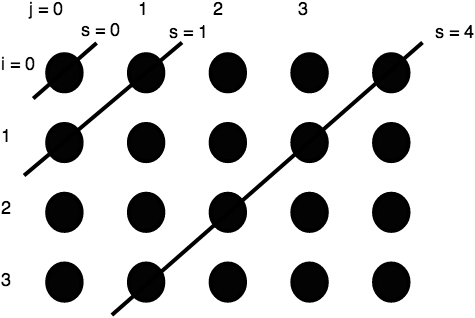
\includegraphics[scale=.4]{ij-by-diagonal}
  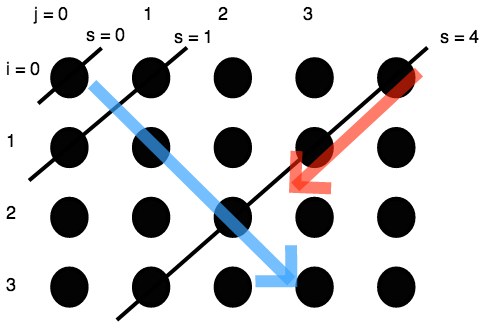
\includegraphics[scale=.4]{ij-by-diagonal-arrow}
  \egroup
  \caption{Traversal of $i,j$ range by $i+j=c$}
  \label{fig:ij-diag}
\end{figure}

For the following exercise, see figure~\ref{fig:ij-diag}.

\begin{exercise}
  \label{ex:ij-product}
  Write a double loop over $0\leq i,j<10$ that prints the first pair
  where the product of indices satisfies $i\cdot j> N$, where $N$~is a
  number your read in. A~good test case is $N=40$.

  Can you traverse the $i,j$ indices such that they first enumerate
  all pairs $i+j=1$, then $i+j=2$, then $i+j=3$ et cetera? Again, you
  should report the first pair $i,j$ for which $i\cdot j>N$. Hint:
  write a loop over the sum value $1,2,3,\ldots$, then find~$i,j$.

  You program should print out both pairs, each on a separate line,
  with the numbers separated with a comma, for instance~\n{8,5}.
\end{exercise}

Another mechanism to alter the control flow in a loop is the
\indextermtt{continue} statement. If this is encountered, execution
skips to the start of the next iteration.

\begin{block}{Skip iteration}
  \label{sl:for-cont}
\begin{verbatim}
for (int var=low; var<N; var++) {
  statement;
  if (some_test) {
    statement;
    statement;
  }
}
\end{verbatim}
Alternative:
\begin{verbatim}
for (int var=low; var<N; var++) {
  statement;
  if (!some_test) continue;
  statement;
  statement;
}
\end{verbatim}
The only difference is in layout.
\end{block}

\begin{block}{While loop}
  \label{sl:while}
  The other possibility for `looping until' is a
  \indextermttdef{while} loop, which repeats until a condition is met.

  Syntax:
\begin{verbatim}
while ( condition ) {
  statements;
}
\end{verbatim}
or
\begin{verbatim}
do {
  statements;
} while ( condition );
\end{verbatim}
The while loop does not have a counter or an update statement; if you
need those, you have to create them yourself.
\end{block}

The two while loop variants can be described as `pre-test' and
`post-test'. The choice between them entirely depends on context. Here
is an example in which the second syntax is more appropriate.

\begin{block}{While syntax 1}
  \label{sl:while2}
  \verbatimsnippet{whiledo}

  Problem: code duplication.
\end{block}

\begin{block}{While syntax 2}
  \label{sl:while3}
  \verbatimsnippet{dowhile}

  The post-test syntax leads to more elegant code.
\end{block}

\begin{exercise}
  \label{ex:interest}
  One bank account has 100 dollars and earns a 5~percent per year interest
  rate. Another account has 200 dollars but earns only 2~percent per
  year. In both cases the interest is deposited into the account.
  
  After how many years will the amount of money in the first account
  be more than in the second?
\end{exercise}

\Level 0 {Exercises}

\begin{exercise}
  \label{ex:pythagoras}
  Find all triples of integers $u,v,w$ under 100 such that
  $u^2+v^2=w^2$. Make sure you omit duplicates of solutions you have
  already found.
\end{exercise}

\begin{exercise}
  \label{ex:collatz}
  The integer sequence
  \[ u_{n+1} = 
  \begin{cases}
    u_n/2&\hbox{if $u_n$ is even}\\
    3u_n+1&\hbox{if $u_n$ is odd}\\
  \end{cases}
  \]
  leads to the Collatz conjecture: no matter the starting guess~$u_1$,
  the sequence $n\mapsto u_n$ will always terminate at~1.

  { \small
  \[ 5\rightarrow 16\rightarrow 8\rightarrow 4\rightarrow 2\rightarrow 1\]
  \[ 7\rightarrow 22\rightarrow 11\rightarrow 34\rightarrow
  17\rightarrow 52\rightarrow 26\rightarrow 13\rightarrow
  40\rightarrow 20\rightarrow 10\rightarrow 5\cdots \]
  }

  (What happens if you keep iterating after reaching~1?)
  
  Try all starting values $u_1=1,\ldots,1000$ to find the values that
  lead to the longest sequence: every time you find a sequence that is
  longer than the previous maximum, print out the starting number.
\end{exercise}

\begin{exercise}
  Large integers are often printed with a comma (US~usage) or a period
  (European usage) between all triples of digits. Write a program that
  accepts an integer such as $2542981$ from the user, and prints it as
  \n{2,542,981}.
\end{exercise}

\begin{exercise}
  \label{ex:rootfind}
  \textbf{Root finding.}
  %
  For many functions~$f$, finding their zeros, that is, the values~$x$
  for which~$f(x)=0$, can not be done analytically. You then have to
  resort to numerical \indexterm{root finding} schemes. In this
  exercise you will implement a simple scheme.

  Suppose $x_-,x_+$ are such that 
  \[ x_-<x_+,\qquad f(x_-)\cdot f(x_+)<0,\]
  that is, the function values are of opposite sign. Then
  there is a zero in the interval~$(x_-,x_+)$. Try to find this zero
  by looking at the halfway point, and based on the function value
  there, considering the left or right interval.
  \begin{itemize}
  \item How do you find $x_-,x_+$? This is tricky in general; if you
    can find them in the interval~$[-10^6,+10^6]$, halt the program.
  \item Finding the zero exactly may also be tricky or maybe
    impossible. Stop your program if $|x_--x_+|<10^{-10}$.
  \end{itemize}
\end{exercise}

\Level 1 {Further practice}

The website
\url{http://www.codeforwin.in/2015/06/for-do-while-loop-programming-exercises.html}
